\identify{Identify the Challenge \& Set Goals: Arm V2.0 ()}
\info{Caleb Bachmeier}{Arm V2.0}{}
\chapterauthor{Caleb Bachmeier}
\textbf{Goal}: We will identify an objective for our robot so that we can address it and build an effective solution
\section*{Problem Statement}
The team wants to create a mechanism that will lift the Rings and put them onto a Neutral Stake, Figure \ref{fig:neutral-stake} "\cite{RECF}"
\begin{figure}[H]
    \centering
    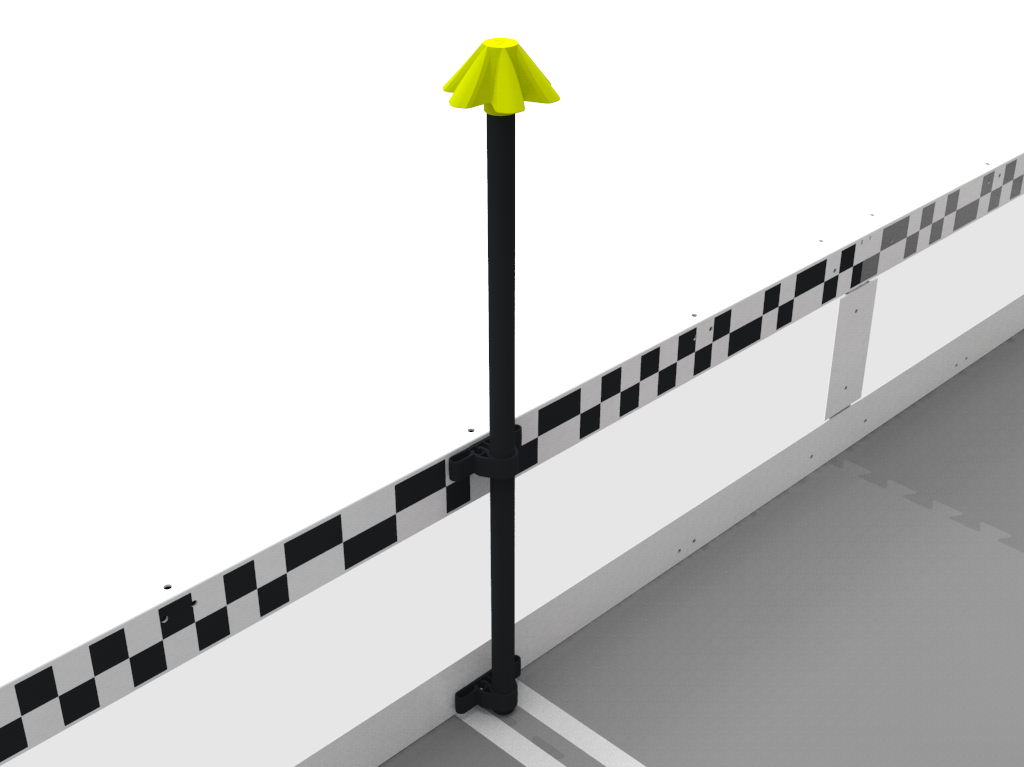
\includegraphics[width=0.5\linewidth]{images/Neutral Stake.png}
    \caption{Neutral Stake}
    \label{fig:neutral-stake}
\end{figure}
\section*{Solution Requirements}
\begin{itemize}
    \item This mechanism would need to use pneumatics, we don't have any motors to spare
    \item This mechanism needs to have at least 70\% accuracy 
    \item We need to stay within the 18 x 18 x 18 space restrictions 
\end{itemize}
\section*{Solution Goals}
\begin{itemize}
    \item We want to create something intuitive and easy for Chase to use
\end{itemize}

\brainstorm{Brainstorm \& Diagram: Arm V2.0 ()}
\info{Caleb Bachmeier}{Arm V2.0}{date}
\chapterauthor{Caleb Bachmeier}
In the past we did a "Victory Arm" design. This worked amazing for its time but wouldn't hold up to today's standard as the VEX "Meta" (The most optimal solution) is always changing.
\section*{Possible Solution - "Lady Brown"} 
A "Lady Brown" is a mechanism that takes a ring off of the top of the intake, and puts it on the Wall Stake. This is shown in \ref with 7686A's Robot \cite{7686a} and \ref with 229V's robot \cite{229V}

\noindent
\textbf{Pros}:
\begin{itemize}
    \item Meta
    \item We can score two rings at once
    \item We wouldn't need to design a redirect 
    \item It is super easy for Chase to use
\end{itemize}
\textbf{Cons}:
\begin{itemize}
    \item Almost every team is using this, so we wouldn't have much to improve or innovate on.
\end{itemize}

\solution{Choose a Solution \& Make a Plan: Arm V2.0 ()}
\info{Caleb Bachmeier}{Arm V2.0}{date}
\chapterauthor{Caleb Bachmeier}
\section*{Choose a Solution}

\section*{Make a Plan}
A YouTube video piqued everyone's interest. The design was a two-ring arm basket with a pivoting end to better conform the rings to the wall stakes. We had also recently seen a design for an arm that can go 360 degrees—useful for tipping mobile goals—and wanted to implement that too. This is shown well in Figure \ref{fig:luke-pivoting-lb} "Luke does robotics" \cite{lukewallstakes} 
\begin{figure}[H]
    \centering
    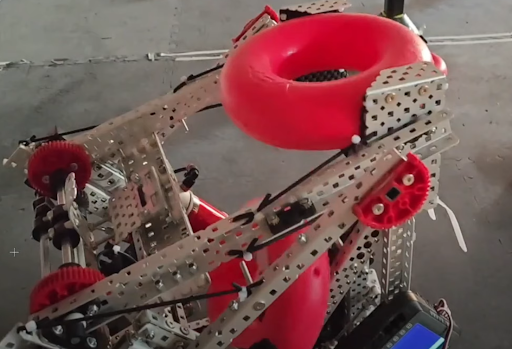
\includegraphics[width=0.5\linewidth]{images/Luke Pivoting LB.png}
    \caption{Pivoting Lady Brown}
    \label{fig:luke-pivoting-lb}
\end{figure}
In order to do as such before building, I started by drawing the geometries in CAD (Ask me for pictures of this). I drew two endpoints and had to find a line for valid intersecting arcs. The center point of the arc would be the pivot location, and the radius would be the arm length.

After creating a very rough draft of what we wanted, I moved the intake in to fit the style of arm we would be using. I had to ensure enough clearance for the hooks while making the top rollers as low-profile as possible. This wasn’t too difficult, as all it took was moving bracing.

\build{Build \& Program: Arm V2.0 ()}
\info{Ian Smith}{Arm V2.0}{February 4th, 2025}
\chapterauthor{Ian Smith}
\section*{Building}
Then, I loosely mounted L-channels to the drivetrain bracing to support the pivot. From that point, I very loosely reattached the mobile goal clamp and mocked-up the axle and arm. (Caleb, you will have to ask me for all my pictures)

Following the team practice on January 30, I worked on getting the motor (66rpm 5.5w) connected to the pivot with gears loosely supporting the arm. The goal here was not to create a definitive design but rather a pseudo-geometry that could be used for later development. Caleb at the prior practice had finished “boxing” the lower intake for better stability. With that done, it was time to start prototyping the intake geometry. I had played with it in CAD for a while but found that it was going to have to be mostly experimental. 

The plan was to prototype the intake geometry in 3D-printed PLA and laser-cut acetal after finding a proper shape. The first prototype would have a hole for where I initially thought the axle might go through for the lower hooks, a 3.5-inch radius circle from the center point of the intake rollers to create the arc, a 60-degree angle, and an “eyeballed” added thickness. The shape ended up being too short, so I had to extend it. I got out the chain for the hooks and found valid positions for the axle. I made note of said positions and adjusted the CAD model. I also found the curvature of the intake ramp to be too aggressive, which caused binding of the lower intake. The arc got extended to have a radius of 4.2 inches, a number calculated for a previous design. I also added some support positions for better stability. (Add pictures of CAD here) 

After light initial testing without the hook, I found the ring would like to wrap around the flex wheel. To solve this, I added flaps to press the ring to the ramp. The only issue: I didn’t have proper material to make a prototype in the moment, so I just modified an earlier intake ramp prototype. After mounting, it immediately fixed the issue. Finally, I mounted the upper intake chain to the ramp. After testing the geometry, it was ready for tuning.

{"originatingScript":"m2","payload":{"guid":"bd5b3fe5-bcb6-4473-8dc3-8775bd7bbea10f21df","muid":"e85d44aa-714f-4310-b8c8-cfba21cef6ea7c9fc6","sid":"6b699a75-bde0-43a5-9186-e6283aeed2ff7a8ca5"}}

\test{Test the Solution: Arm V2.0 ()}
\info{author}{Arm V2.0}{date}
\chapterauthor{}
\section*{Test the Solution}
